\documentclass[12pt]{article}    
\usepackage[left=2cm, right=2cm, top=2cm, bottom= 2cm]{geometry} 
\usepackage{graphicx,epsfig,verbatim,enumerate}
\usepackage{amssymb,amsmath,amsthm,amsbsy}
\usepackage{ifthen}
\usepackage{morefloats}
\usepackage[hidelinks]{hyperref}
%\hypersetup{colorlinks=true, linkcolor=blue}
\usepackage{cite}
\usepackage{color}
\usepackage{textcomp}
\usepackage{float}

\newcommand{\todo}[1]{\noindent\textcolor{blue}{{$\Box$ #1}}}

\title{Project Proposal}
\date{\today}
\author{Luke Trinity and Nat Shenton \\  CS 254}

\begin{document} 
\maketitle
\section{Introduction}

Online sources of high resolution images including Google, Image-net \cite{deng2009imagenet}, and Flickr are providing new opportunities to explore applications of image categorization using computer vision. One interesting application in the field of fine-grained image classification is identification of dog breed. Dogs faces are considered to be highly differentiable for each breed, which makes classification an approachable problem.  However, the work is challenging due to the varying combinations of facial characteristics and color patterns between species, as well as intra-class variation within a single species. Another aspect of the problem that makes it more complicated is the presence of humans and man-made backgrounds, which are not as common in other animal datasets. In addition, many attempts to classify dog breeds fail to corroborate the results with actual DNA evidence. Our approach will be to utilize an existing dog breed image classification dataset \cite{khosla2011novel}, in combination with a novel dataset that includes paired DNA test results and photos \cite{voith2009comparison}, to  classify non-pure bred dog breeds. 

\section{Problem Definition and Algorithm}

\subsection{Task Definition}

The task is to take dog images where each image is labeled either mixed or pure breed and use them to train an algorithm to classify an unseen photo based on whether the dog is mixed or pure.  An important part of training our neural network is to normalize the input images.  Each input image is defined as a matrix of $250\times 250\times3$.  The output of this algorithm, will either be a mixed or pure bred dog. This is an interesting problem as it could provide dog owners an easy way to classify if their dog is a pure bred or mixed, and combines multiple methods of machine learning. It could be an exciting way to start a conversation and help people learn about different breeds of dogs, and how they are mixed. The final goal for this task would allow for a dog owner to upload a picture of their dog to a website or app and then the machine learning algorithm will classify their dog as a percentage of each breed. 

\subsection{Dataset}

The Stanford Dogs Dataset has 20,580 images each classified into one of 120 classes of dog breed. \cite{khosla2011novel} Each image also has an associated bounding box identifying the location of the dog within the photo. The mixed-breed DNA identified dog photo dataset from Voith et al. \cite{voith2009comparison} has 20 images, each paired with DNA percentage breakdown of dog breed. The final mixed breed data set a combination of the top 25 mixed dog breeds from dogfinder.com, and crowdsourcing bring the total up to \textbf{number of mixed dogs} pictures.  The final dataset was obtained by a random sampling of pure bred dogs fromthe Standard dataset equal to the length of the amount of dogs form the Stanford Dogs Dataset.  This created a dataset of \text{total number of dogs}. There are no associated bounding boxes for the Voith dataset \cite{voith2009comparison}. 

\subsection{Algorithm Definition}

First, we utilize the Resnet50 convolutional neural network as it achieves roughly 80\% accuracy on the Standford dog dataset. This pretrained neural network gives a classification accuracy high enough that it should classify an image of a purebred dog correctly.  This pretrained convolutional neural network is trained on Google's ImageNet which contains the Stanford Dogs dataset. By feeding images from the mixed dog breed dataset into this pretrained neural network, the network gives the output as the probability of each dog breed. The output contains the probabilities of 1000 labels, and the algroithm will only take the labels with the top 4 highest probabilities. From here principal component analysis is used to take the four prediction outputs from the pretrained convolutional neural network down to two features.  With these two features as the input classes, a sweep of three classification methods were used SVM, random forrest, and a neural network.

For the SVM classifier two techniques are used.  The first being a random sweep over a linear kernel with a C values randomized over an exponential distribution starting at 1000, and $\gamma$ values randomized over an exponential distribution starting at 2.  Other SVM algorithm has the same C and $\gamma$ sweeps but also randomly chooses a Radial Basis Function kernel or a polynomial kernel.  The random forest algorithm looks at a forest of 10 trees. Lastly the neural network uses an architecture of 3 hidden fully connected layers with the ReLu activation function.  The first layer contains 48 nodes, the second 24 nodes, and the third 4 nodes. The output layer contains one node with a sigmoid activation function.  The model was then compiled with the Adam gradient descent optimizer, and binary cross-entropy as the loss function.  The neural network was trained over 300 epochs.

Cross validation is run on each model type to fit the optimal algorithm in terms of accuracy score. These four types of models were each chosen to run randomly over 200 time steps to find the optimal model from each model type.  Of these four the model with the highest accuracy score in the validation stage is chosen to be the final model.



\begin{figure}[H]
\centering{
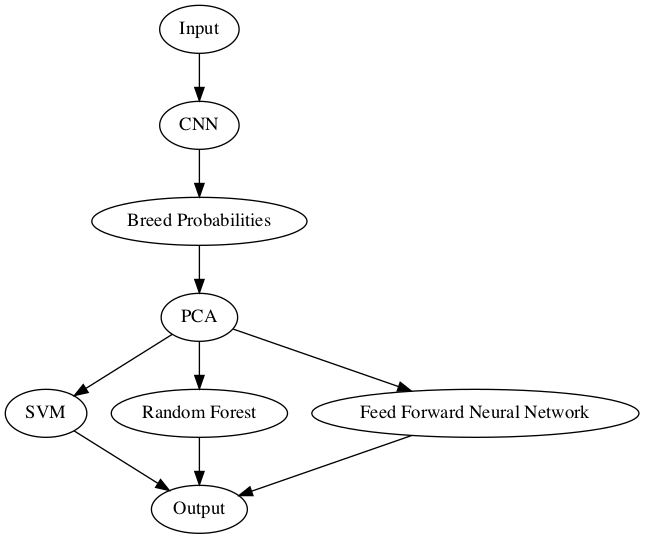
\includegraphics[width=0.7\textwidth]{modelgv}
}
\end{figure}
%convert each of the images in the Stanford Dogs dataset \cite{khosla2011novel} into a single feature vector based on the trimmed height and width of the images and the (r,g,b) values in each cell. We  then pair the images with their associated class labels, and utilize a neural network as a black box to train our model to accurately predict the class of our test images. Later in the semester we hope to unbox the neural network with more advanced knowledge to achieve better accuracy. One method we will work to implement, which was utilized by both Kohsla et al. \cite{khosla2011novel} and Liu et al. \cite{liu2012dog}, is scale-invariant feature transform (SIFT). This algorithm detects and describes local features in images by finding candidate matching features based on Euclidean distance of feature vectors.  \cite{lowe2004distinctive} After achieving a high level of accuracy classifying pure-bred dogs, we plan to introduce our other dataset \cite{voith2009comparison} that carries interesting practical concerns in our implementation of SIFT. Here we will attempt to classify mixed breed dogs using images annotated with precise DNA testing of breed composition. Hopefully we can augment this dataset with more samples by reaching out to different labs. This is an interesting computer vision problem because dogs often share features, whether it be color patterns or facial structure, that lead to breed misrepresentation.  Training an algorithm in this capacity could lead to novel conclusions related to classifying a dog as purebred or a mixed breed, hopefully we can leverage innovations such as Googles Opensource API, a way to detect objects that could increase our accuracy. 
 
\section{Experimental Evaluation}

\subsection{Methodology}

We first generated our dataset by specifying only two breeds to classify. Each image for the corresponding dog breeds was linked with its associated bounding box, which specifies exactly where in the image the dog is located. Then, each image was converted into an array of dimension $(250,250,3)$. At this point it is important to note that the dataset is balanced, but not perfectly, meaning there are not equal numbers of images for each dog breed in the dataset but they are very similar ($\approx 150$ per breed). Having obtained our data matrix for two breeds, we normalized the pixel values from $(0,255)$ to $(0,1)$ by dividing each pixel by 255. The target vector is simple to generate, with $0$ for the first breed and $1$ for the second. We then passed each one of our images through a simple Keras neural network with three layers, using two epochs as our initial number of iterations to train the weights. Having accomplished our initial basic goal of classification, we then sought to increase the number of breeds our network could classify. For this we modularized our code to classify $N$ breeds, where we increased $N$ until our algorithm resulted in a memory error when $N=8$. If our algorithm had not resulted in a memory error, it should hypothetically work for all the breeds in our dataset.

By using the r

\subsection{Results}

Here we display the results of training our network on an increasing number of breeds, and the resulting decrease in accuracy. The drop in accuracy is expected, because the task gets harder as there are more potential breeds any of the test images could potentially be classified as. Important to note here is that we did use cross-validation in reporting our accuracy, and that in this case, accuracy is a weighted combination of precision and recall from the Keras package. 

 \begin{figure}[H]
 \centering
  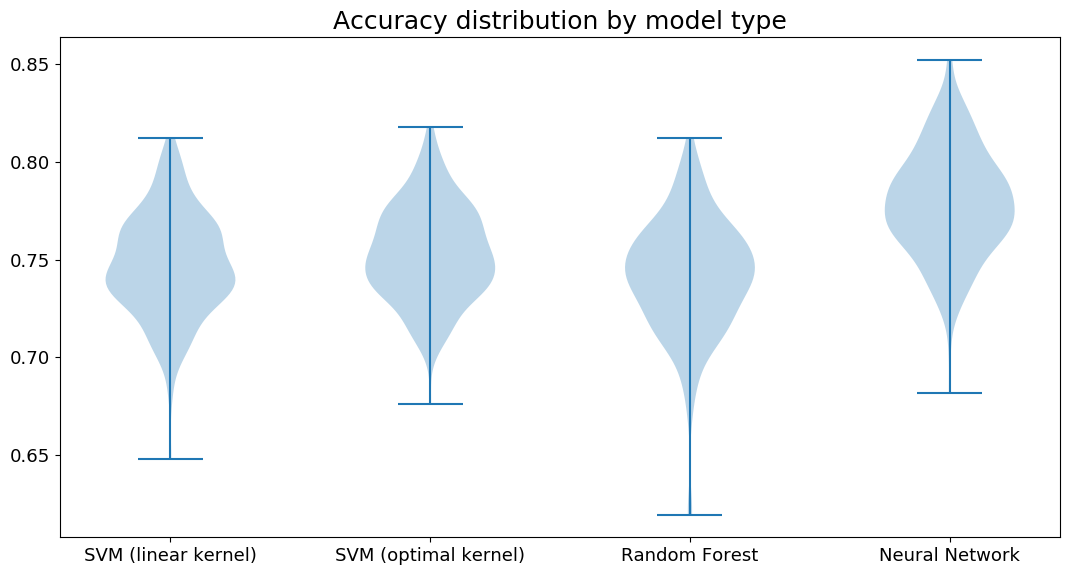
\includegraphics[width=0.7\textwidth]{testOut}
  \caption{Keras model accuracy over increasing number of breeds trained on, where 0 on the x-axis corresponds with the baseline of 2 breeds trained on.}x
  \end{figure}
  
\subsection{Discussion}

Interestingly, the accuracy increased slightly from $N=6$ to $N=7$. This may not be significant, but in the future we can average over multiple runs to determine if the trend is consistent. It is also possible that with more breeds to train on, the model could become more accurate because certain breeds are very unique and easy to classify. We believe this is an excellent output, with the potential to scale easily and help us accomplish our intermediate goal of classifying any pure bred dog, before moving on to mixed breeds classification. The algorithm has great potential for improvement, with only the barebones framework currently in place. 

\section{Related Work}

In the initial article utilizing the novel dataset by Khosla et al. \cite{khosla2011novel}, the mean accuracy reached 22\% when 100 training images were utilized within the SIFT methodology. Liu et al. \cite{liu2012dog} reached 69\% accuracy, with greater success than Khosla et al. \cite{khosla2011novel} due to their partially localized approach.  We hope to leverage the bounding boxes and augment the work of Liu et al. \cite{liu2012dog}, possibly improving on their methodology to achieve higher accuracy. Several bounding box approaches are currently being reviewed, although all are endlessly modifiable from simple image segmentation. One is a slight adaptation to a method often employed for training algorithms to images of different shade and dimension called DeepCut.  \cite{rajchl2016deepcut} There are several standard variations on the basic DeepCut methodology, which hones in on the nature and dimension of the bounding in a cookie-cutter, traced-out way as opposed to any kind of geometric shape. A very similar methodology is known as GrabCut which does not need to even be a single, continuous cookie-cutter-style line bounded around a desired segment of an image. GrabCut is standardly designed to grab multiple disparate segments of an image at once for a single, desired analysis. In addition to one of these approaches or some modification thereof, we plan to incorporate some aspect of KL Loss to account for localization uncertainty which could greatly assist with interference from background objects such as people, buildings, trees, etc. \cite{he2019bounding} There are, of course, a number of other modifiable ‘standard’ or ‘familiar’ combinations of approaches to deal with bounding and uncertainty to also be explored. Even so, most will lead to an approximately similar result if implemented correctly. Deep/GrabCut is simple and can narrow the selected image segment in a convenient, efficient manner. KL Loss will be further researched and incorporated to deal with expected shading difficulties, image blurring and background/foreground image ‘noise’.

\section{Next Steps}

The initial Neural network trained using Keras shows the classification of dog breeds gets worse and worse as more breeds are introduced. From these results there are two main directions this project will have to go.  The first is it move this project onto the VACC, which should avoid the memory error when running any more than a 7 breed classification which occurred on the local machine.  We will test the performance of both the Bluemoon and DeepGreen supercomputer clusters to scale the model from the 7 breed classification to the 120 breed classification.  The model will return the prediction probability vector for all breeds. This will be Luke's main task.

The second task will be to improve the model.  Using cross validation, the pre-weighted neural networks from the Keras libraries will be used to improve the model. Keras has an extensive library of pre-weighted networks specifically designed from image classifications. This will include the tuning of hyper parameters to improve the prediction probability through cross validation, as well as going inside the black box that is the neural network and experimenting with different numbers and types of sequential layers.  This will be Nat's main task.  

Once the algorithm has been optimized, the final step of the project will be a user interface where a user will upload an image of their dog, and the algorithm will return the prediction probability.  This will either be done with a simple HTML page or using the Unity platform. 

\section{Code and Dataset}

The code can be found in our github repo: \url{https://github.com/nshenton/CS_251_DogProject}.  Please see the Readme in the repo for more information.  The Stanford Dogs Dataset can be downloaded from this page: \url{http://vision.stanford.edu/aditya86/ImageNetDogs/}.

\section{Conclusion}

Here we have described our barebones methodology and presented intermediate results. Our path forward will involve a team effort of improving the accuracy of our model, and leveraging the technologies of the VACC. We believe our final product will be interesting and a great conversation starter for dog lovers and machine learning enthusiasts alike. Our elavator pitch is simple, wouldn't you like to upload a photo of your dog and see what breeds it could potentially be? Looking past this semester, it would be a long-term goal to incorporate user feedback into the training of the model, i.e. having users rate the predictions for how accurate they are perceived to be. 

\bibliography{dogbib}{}
\bibliographystyle{ieeetr}

\end{document}    